\chapter{Experimental Protocol and Results}
\label{ch:results}
\begingroup
\renewcommand{\figfile}[5]{\begin{figure}[!htbp]\centering\includegraphics[width=#2\linewidth]{#1}\caption[#3]{#4}\label{#5}\end{figure}}

\section{Evaluation objectives and selected systems}
The final evaluation examines the complete detector on Modena and L-Town. It measures attack detection and false alarms across fitted models and generated sources, including the families on which performance remains weaker. Both networks contribute to the result: Modena evaluates the selected architecture in its principal development setting, while L-Town tests a network with a larger and different hydraulic structure.

Modena retains the confirmed Stage-E system; L-Town retains the confirmed history extension within General. Chapter~\ref{ch:architecture} specifies these network-specific implementations. The following comparisons assess their final decisions.

The core campaign contains three comparisons. The original Modena confirmation compares the previous guarded system, a threshold-only alternative and the Stage-E candidate on the same fresh sources. The L-Town history confirmation compares the selected history system with its matched no-history baseline. The final extension adds five model seeds to each selected design and summarizes all ten fits. Their baselines and source sets differ, and the tables identify the relevant population at each step [\evid{E1}, \evid{E8}, \evid{E2}]. A subsequent single-classifier comparison addresses complexity under the retained benchmark in Section~\ref{sec:singlebaseline}.

\section{Frozen experimental procedure}
\subsection{Training, calibration and assessment}
The final benchmark retains the observation and attack settings defined in Chapter~\ref{ch:benchmark}. Scenarios span 168 hours with hourly observations, pressure and flow missing probabilities remain 0.50, and the generator distribution, attack severity and scenario splits are preserved. The prediction target is an actually received pressure endpoint after feature warm-up. Missing readings are excluded from the decision population through the availability masks.

Training fits the normal reference and the supervised components. Source-held predictions supply the integration heads with expert outputs from sources excluded from the corresponding expert fit. Calibration selects operating points using the permitted search procedure and protection criteria. Evaluation follows the freezing of the selected models and rules. This separation is especially relevant to the history comparison, where a feature update changes the score distribution and therefore requires a calibrated operating point.

The two networks use different training and calibration collections. Modena has 110 training and 99 calibration scenarios; L-Town has 120 and 96, respectively. The corpus definitions, including Modena's shared source 811 with disjoint scenario subsets, are given in Table~\ref{tab:corpora}. Evaluation uses six source datasets per network, each containing 24 scenarios. Thus each fitted model is assessed on 144 scenarios, and the same scenarios recur across model seeds within that network.

The original Modena selection uses the Stage-E calibration procedure. In L-Town, the original combination of clean-FPR and absolute family-floor constraints was infeasible. Before L-Town evaluation, the campaign amended the procedure to retain the clean-FPR budget of 0.005 and relative family protection while reporting the unmet absolute floors. The selected L-Town rule satisfies this amended procedure; the original replay floor remains unmet [\evid{E1}].

The initial research goal for L-Town replay F1 was 0.80; this was revised to 0.75 during development when the original goal proved difficult to attain. These values specify research performance goals rather than alarm-score thresholds.

The later protected-history protocol adds its own explicit checks. It requires a replay improvement while protecting pooled performance, clean FPR and the other families, with specified tolerances at model and source levels. The external specialist pipeline is preserved. The full-history variant is selected on calibration and frozen before its original fresh confirmation. The failed earlier General-only noise-protection gate remains a development result, as described in Chapter~\ref{ch:development}; the full-system result concerns a separately specified intervention [\evid{E8}].

\subsection{From five fits to ten}
The original confirmation uses model seeds 701--705. The extension adds seeds 706--710, refitting the stochastic components with the selected recipe. It retains the network-specific calibration algorithms and freezes all added models and rules across both networks before extension evaluation. The added seeds use the existing six evaluation sources. This measures sensitivity to fitting randomness conditional on those sources, while preserving the original confirmation chronology [\evid{E2}].

For Modena, the evaluation sources are 40811, 41811, 42811, 43811, 44811 and 45811. For the selected L-Town history system they are 110811, 111811, 112811, 113811, 114811 and 115811. The \emph{original locked test} denotes four whole scenarios (0, 1, 8 and 20) reserved from the initial 24-scenario Modena source 811. The original split was selected using scenario-level family coverage and observed replay-positive availability, independently of detector scores. Those scenarios remained excluded from fitting, calibration and the reported evaluation. The later campaign defined separate generator-source collections for confirmation and repeated-fit assessment, so the results reported here concern those collections; no performance estimate on the original reserved split is claimed. All ten fits are retained in the final result, including their source-level variation; the reported system is evaluated as individual fitted realizations, without combining their predictions into an ensemble.

The reported endpoint scores include specialist decisions made by $t+3$, alongside General's immediate decisions at time $t$. Early warning supplies network-time context to verification.

\section{Aggregation and uncertainty}
Let $M_{r,s}$ denote a metric for model seed $r$ and source $s$, within one network. The final reported mean is
\begin{equation}
 \overline M=\frac{1}{10\cdot6}\sum_{r=1}^{10}\sum_{s=1}^{6}M_{r,s}.
 \label{eq:cellmean}
\end{equation}
For pooled F1, each $M_{r,s}$ is computed from the true-positive, false-positive and false-negative counts over all retained endpoints in that cell. Those F1 values are then averaged. Since F1 is nonlinear, this differs from first merging counts across all fits and computing one F1. Reusing an endpoint under ten fitted models also does not create ten independent observations of the underlying hydraulic process.

Metric populations follow Chapter~\ref{ch:benchmark}: family scores cover family-coded periods, pooled F1 covers all retained endpoints, and clean FPR covers clean periods. Family macro F1 gives equal weight to the five families. Tables express clean FPR as a percentage; a rate of 0.000584 appears as 0.0584\%.

Equation~\eqref{eq:marginalmeans} defines two marginal summaries of the variation:
\begin{equation}
 \overline M_{r,\cdot}=\frac{1}{6}\sum_s M_{r,s},\qquad
 \overline M_{\cdot,s}=\frac{1}{10}\sum_r M_{r,s}.
 \label{eq:marginalmeans}
\end{equation}
The sample standard deviation of the ten model means describes fit-to-fit variation after averaging over sources. The sample standard deviation of the six source means describes differences between generated collections after averaging over fitted models. Neither is the standard error of 60 independent datasets. Cell ranges and counts below reference levels complement these summaries by showing outcomes hidden by the overall mean.

For matched interventions, the reported difference is
\begin{equation}
 \overline\delta=\frac{1}{|\mathcal P|}\sum_{(r,s)\in\mathcal P}
 \left(M^{\mathrm{candidate}}_{r,s}-M^{\mathrm{baseline}}_{r,s}\right),
 \label{eq:paireddifference}
\end{equation}
where $\mathcal P$ is the set of evaluated pairs. Modena's original confirmation contains 30 pairs, and the final L-Town history comparison contains 60. Positive-pair counts describe the consistency of the observed intervention. The analysis reports these descriptive quantities with the source structure visible, rather than treating repeated endpoints or model fits as independent replications for a significance claim. Differences are computed from unrounded metrics and may therefore differ slightly from differences between the displayed values.

\section{Final results on both networks}
\begin{table}[tbp]
\centering\small
\caption[Final ten-seed results on both networks]{Final selected-system means over 60 model/source cells per network. F1 is on the 0--1 scale; clean FPR is expressed as a percentage.}
\label{tab:finalmeans}
\begin{tabular}{@{}lrr@{}}
\toprule
Metric & Modena & L-Town\\
\midrule
Random & 0.9549 & 0.9920\\
Replay & 0.9283 & 0.7312\\
Drift & 0.8274 & 0.8990\\
Noise & 0.8439 & 0.9279\\
Targeted & 0.9680 & 0.9918\\
Family macro F1 & 0.9045 & 0.9083\\
Pooled F1 & 0.8669 & 0.8950\\
Clean FPR (\%) & 0.0584 & 0.0550\\
\bottomrule
\end{tabular}
\end{table}

Table~\ref{tab:finalmeans} reports the selected systems. Modena achieves mean pooled F1 of 0.8669 and family macro F1 of 0.9045. L-Town achieves 0.8950 and 0.9083, respectively. Their clean FPRs are 0.0584\% and 0.0550\%. Expressed as normalized reading-level rates, these correspond to approximately 58.4 and 55.0 alarms per 100,000 clean evaluated endpoints.

The family profiles differ substantially despite their similar macro scores. Modena is strongest on random and targeted corruption, followed by replay. Drift and noise are its weaker families. L-Town is strongest on random and targeted corruption and retains high drift/noise scores, while replay is substantially lower. Figure~\ref{fig:finalfamilies} compares the five family scores in each network.

\figfile{results_families.pdf}{1.0}{Final family-level performance on both networks}{Mean family-conditioned F1 of the selected systems, each evaluated across ten model seeds and six source datasets. The dashed reference marks 0.80. Values summarize the 60 model/source cells within each network.}{fig:finalfamilies}

\FloatBarrier
\section{Modena: improved precision with a measured trade-off}
\subsection{Matched confirmation of the integrated system}
The original Stage-E confirmation provides the controlled evidence for the major pooled-F1 improvement. All three arms use the same five model seeds and six fresh sources. Table~\ref{tab:modenapaired} reports their mean scores. The candidate increases pooled F1 from 0.6863 to 0.8672, a paired gain of 0.1809, whereas the threshold-only alternative reaches 0.6998. The candidate outperforms the baseline in pooled F1 in all 30 cells [\evid{E1}].

\begin{table}[tbp]
\centering\small
\caption[Original matched Modena confirmation]{Original Modena confirmation: five model seeds and six fresh sources, with all three arms scored on the same 30 cells. The final ten-seed selected-system mean is reported separately in Table~\ref{tab:finalmeans}.}
\label{tab:modenapaired}
\begin{tabular}{@{}lrrrr@{}}
\toprule
Metric & Baseline & Threshold only & Candidate & $\Delta$ candidate\\
\midrule
Random & 0.9513 & 0.9551 & 0.9542 & +0.0029\\
Replay & 0.9030 & 0.9071 & 0.9280 & +0.0250\\
Drift & 0.8333 & 0.8494 & 0.8262 & -0.0071\\
Noise & 0.8506 & 0.8428 & 0.8455 & -0.0051\\
Targeted & 0.9605 & 0.9634 & 0.9674 & +0.0069\\
Pooled F1 & 0.6863 & 0.6998 & 0.8672 & +0.1809\\
Clean FPR (\%) & 0.4262 & 0.3997 & 0.0574 & -0.3687\\
\bottomrule
\end{tabular}
\end{table}


The confusion counts explain the scale of this improvement. Summed across the repeated evaluations, baseline true positives are 79,809, false positives 62,722 and false negatives 10,156. The candidate yields 76,532 true positives, 9,910 false positives and 13,433 false negatives. False positives decrease by 84.2\%, while true positives decrease by 4.1\%. The resulting precision gain more than compensates for the reduced recall in pooled F1. These sums describe repeated model evaluations on shared sources; they are used here to explain the error balance, not as counts of distinct physical incidents.

The family-level effects are more selective. Random improves by 0.0029, replay by 0.0250 and targeted by 0.0069. Drift decreases by 0.0071 and noise by 0.0051. These losses fall within the recorded 0.01 mean-protection tolerance, but they are systematic: drift declines in 22 of the 30 cells and noise in 25. The improved precision comes with small but frequent losses in the specialized families.

The earlier EVAL-3 pooled F1 of 0.6515 explains why background alarms became a development priority. Its evaluation population differs from the fresh Stage-E comparison. The matched gain attributed to the later intervention is 0.8672 minus 0.6863. The threshold-only arm further shows that a new operating point on its own accounts for only a small part of that change. The larger intervention combines the selected calibration procedure with verification and early-warning context; the experiment evaluates that package, rather than separately identifying the contribution of each added head.

\subsection{The final ten-seed Modena profile}
With ten model seeds, Modena's pooled mean is 0.8669, close to the original five-seed value of 0.8672. Random, replay and targeted retain means of 0.9549, 0.9283 and 0.9680. Drift and noise average 0.8274 and 0.8439. The added fits reproduce both the strong aggregate result and the weaker drift and noise performance.

All family means exceed 0.80, but the source-level pattern is uneven. Drift falls below 0.80 in 19 of the 60 cells and noise in ten. Their minima are 0.7652 and 0.7811. In contrast, every random, replay and targeted cell remains above 0.80. The family averages therefore conceal some weaker outcomes on individual sources and fits.

These weaker scores are structured by source. Section~\ref{sec:sourceperformance} reports their source averages alongside the corresponding L-Town profile.

\section{L-Town: protected history improves the complete detector}
\subsection{Matched full-system effects}
The selected L-Town intervention supplies received-pressure history to all five internal General components and its internal router, while preserving the external specialist pipeline. In its original fresh confirmation, mean replay F1 increases from 0.7064 to 0.7303 and pooled F1 from 0.8895 to 0.8951. All 30 replay differences are positive, and the predeclared protection checks pass. These results establish the original confirmation of the history design [\evid{E8}].

The final ten-seed comparison extends the same selected recipe across model randomness. Table~\ref{tab:historypaired} reports the corresponding 60-cell matched baseline and history means. Replay increases by 0.0247, from 0.7065 to 0.7312. Pooled F1 increases by 0.0088, from 0.8862 to 0.8950. Both differences are positive in all 60 cells. The candidate's stable pooled mean across the original and added seeds is reported in Table~\ref{tab:extension}; the changed paired gain reflects the fitted baseline as well as the candidate.

\begin{table}[tbp]
\centering\small
\caption[Final matched L-Town history comparison]{Final matched L-Town history comparison, averaged over 60 model/source cells. Both systems use the preserved external specialist pipeline. FPR changes are percentage points.}
\label{tab:historypaired}
\begin{tabular}{@{}lrrr@{}}
\toprule
Metric & No-history baseline & Full history & Difference\\
\midrule
Random & 0.9893 & 0.9920 & +0.0026\\
Replay & 0.7065 & 0.7312 & +0.0247\\
Drift & 0.8976 & 0.8990 & +0.0014\\
Noise & 0.9258 & 0.9279 & +0.0021\\
Targeted & 0.9890 & 0.9918 & +0.0027\\
Pooled F1 & 0.8862 & 0.8950 & +0.0088\\
Clean FPR (\%) & 0.0627 & 0.0550 & -0.0077\\
\bottomrule
\end{tabular}
\end{table}


All four other family means also improve. Random gains 0.0026, drift 0.0014, noise 0.0021 and targeted 0.0027. Mean clean FPR decreases from 0.0627\% to 0.0550\%, approximately a 12.3\% relative reduction. The replay gain is accompanied by improvements in the other family means and the overall error balance.

Some individual comparisons show small losses. Drift improves in 49 cells and targeted in 58; random and noise improve in all 60. The largest individual other-family loss is approximately 0.0009 F1. Clean FPR decreases in 40 cells, increases in 19 and is unchanged in one, even though its overall mean falls. The protection criteria apply to the aggregate and source-level results; they allow some losses in individual fits.

\figfile{results_tradeoffs.pdf}{1.0}{Family effects of the matched final-design interventions}{Mean paired family-F1 changes for the original Modena Stage-E confirmation and the final L-Town history comparison. The panels use their own matched baselines and contain 30 and 60 cells, respectively. Green bars indicate gains and red bars losses.}{fig:interventioneffects}

Figure~\ref{fig:interventioneffects} contrasts the interventions: Modena's large precision gain carries drift/noise losses, whereas L-Town's smaller pooled gain accompanies positive means for every family.

\subsection{The remaining replay limitation}
L-Town replay is improved but remains the limiting family. Its final mean is 0.7312, below the later 0.75 objective and the earlier 0.80 reference. Individual cell scores range from 0.6947 to 0.7657. Fifty of the 60 cells are below 0.75, and all are below 0.80. In contrast, random, drift, noise and targeted exceed 0.80 in every final cell.

Section~\ref{sec:sourceperformance} reports replay performance separately for each evaluation source.

\FloatBarrier
\section{Variation across models and sources}
\subsection{Descriptive spread}
Table~\ref{tab:variation} separates model and source variation. For Modena pooled F1, the model-mean SD is 0.0034 and the source-mean SD is 0.0118. For L-Town they are 0.0013 and 0.0109. In both networks the spread between source means is larger than the spread between model means. These marginal summaries describe the observed collections; they are not an additive decomposition into independent variance components.

\begin{table}[tbp]
\centering\small
\caption[Model and source variation of the selected systems]{Descriptive variation of the selected systems. Model SD is the sample standard deviation of ten six-source means; source SD is that of six ten-model means. The range covers all 60 cells. FPR entries use percentage units.}
\label{tab:variation}
\begin{tabular}{@{}llrrr@{}}
\toprule
Network & Metric & Model SD & Source SD & Cell range\\
\midrule
Modena & Random & 0.0041 & 0.0095 & 0.9366--0.9748\\
 & Replay & 0.0022 & 0.0184 & 0.8971--0.9605\\
 & Drift & 0.0056 & 0.0422 & 0.7652--0.8967\\
 & Noise & 0.0032 & 0.0349 & 0.7811--0.8992\\
 & Targeted & 0.0025 & 0.0109 & 0.9394--0.9804\\
 & Pooled F1 & 0.0034 & 0.0118 & 0.8419--0.8896\\
 & Clean FPR (\%) & 0.0084 & 0.0077 & 0.0429--0.0941\\
L-Town & Random & 0.0002 & 0.0011 & 0.9893--0.9941\\
 & Replay & 0.0050 & 0.0173 & 0.6947--0.7657\\
 & Drift & 0.0021 & 0.0291 & 0.8436--0.9317\\
 & Noise & 0.0012 & 0.0085 & 0.9039--0.9388\\
 & Targeted & 0.0002 & 0.0011 & 0.9891--0.9940\\
 & Pooled F1 & 0.0013 & 0.0109 & 0.8785--0.9081\\
 & Clean FPR (\%) & 0.0024 & 0.0026 & 0.0470--0.0619\\
\bottomrule
\end{tabular}
\end{table}


Figure~\ref{fig:modelvariation} displays the individual fitted-model means for pooled F1 and replay. The horizontal lines give the final overall means, and the division after seed 705 identifies the extension. Each point already averages six source datasets. Modena's replay varies relatively little across these model averages, while its pooled performance is more sensitive to the fitted realization. L-Town's pooled model means are tightly grouped, with more visible variation in replay. The distinction is consistent with replay remaining the difficult family even when the aggregate result is stable.

\figfile{results_model_variation.pdf}{1.0}{Variation across the ten fitted models}{Selected-system model means, each averaging the same six sources within its network. The vertical dotted line separates the original five seeds from the added five. Horizontal lines mark the overall means. Panel axes use different restricted ranges to make fitting variation visible.}{fig:modelvariation}

Table~\ref{tab:extension} compares the two five-seed groups directly. Modena pooled F1 changes from 0.8672 to 0.8667; L-Town changes from 0.8951 to 0.8949. The largest family shift between the two groups is Modena noise, which decreases from 0.8455 to 0.8422. L-Town replay increases from 0.7303 to 0.7320. The extension therefore preserves the broad family profile and pooled performance of the originally selected systems.

\begin{table}[tbp]
\centering\small
\caption[Original and added model-seed means]{Selected-system means for the original five model seeds and the added five. Each group averages 30 cells on the same six sources within its network. Clean FPR is expressed as a percentage.}
\label{tab:extension}
\begin{tabular}{@{}lrrrr@{}}
\toprule
Metric & Modena 701--705 & 706--710 & L-Town 701--705 & 706--710\\
\midrule
Random & 0.9542 & 0.9557 & 0.9920 & 0.9919\\
Replay & 0.9280 & 0.9286 & 0.7303 & 0.7320\\
Drift & 0.8262 & 0.8286 & 0.8986 & 0.8993\\
Noise & 0.8455 & 0.8422 & 0.9282 & 0.9275\\
Targeted & 0.9674 & 0.9686 & 0.9918 & 0.9918\\
Pooled F1 & 0.8672 & 0.8667 & 0.8951 & 0.8949\\
Clean FPR (\%) & 0.0574 & 0.0594 & 0.0548 & 0.0551\\
\bottomrule
\end{tabular}
\end{table}


\subsection{Source-dependent performance}
\label{sec:sourceperformance}
Table~\ref{tab:sourcemeans} gives source-level replay, drift, noise and pooled means; Figure~\ref{fig:sourcevariation} shows every family. Modena drift averages 0.7747 on source 44811 and 0.7922 on 42811, compared with 0.8879 on 41811. Noise is weakest on 43811 at 0.7882. L-Town replay ranges from a source mean of 0.7029 on 110811 to 0.7539 on 115811. These differences remain after averaging ten fits.

\begingroup
\let\originaltable\table
\renewcommand{\table}[1][]{\originaltable[!htbp]}
\begin{table}[tbp]
\centering\small
\caption[Source-level means across ten models]{Source-level means across ten fitted models. Source identifiers refer to separate generated scenario collections within each network.}
\label{tab:sourcemeans}
\begin{tabular}{@{}llrrrr@{}}
\toprule
Network & Source & Replay & Drift & Noise & Pooled F1\\
\midrule
Modena & 40811 & 0.9025 & 0.8110 & 0.8411 & 0.8693\\
Modena & 41811 & 0.9357 & 0.8879 & 0.8950 & 0.8851\\
Modena & 42811 & 0.9405 & 0.7922 & 0.8308 & 0.8508\\
Modena & 43811 & 0.9535 & 0.8504 & 0.7882 & 0.8708\\
Modena & 44811 & 0.9201 & 0.7747 & 0.8544 & 0.8579\\
Modena & 45811 & 0.9173 & 0.8481 & 0.8538 & 0.8677\\
L-Town & 110811 & 0.7029 & 0.8814 & 0.9304 & 0.8821\\
L-Town & 111811 & 0.7297 & 0.9067 & 0.9121 & 0.8914\\
L-Town & 112811 & 0.7403 & 0.8492 & 0.9346 & 0.8831\\
L-Town & 113811 & 0.7229 & 0.9277 & 0.9272 & 0.9047\\
L-Town & 114811 & 0.7372 & 0.9075 & 0.9358 & 0.9025\\
L-Town & 115811 & 0.7539 & 0.9214 & 0.9271 & 0.9063\\
\bottomrule
\end{tabular}
\end{table}

\endgroup
\figfile{results_source_variation.pdf}{1.0}{Family performance across evaluation sources}{Family F1 averaged over ten model seeds for each source. The common color scale spans 0.70--1.00; printed values give the individual source means. Source identifiers distinguish scenario collections, and matching row positions across networks do not denote matched hydraulic scenarios.}{fig:sourcevariation}

Source-mean pooled F1 ranges from 0.8508 to 0.8851 in Modena and from 0.8821 to 0.9063 in L-Town. These values average ten fits; the cell ranges also reflect fitting variation.

\FloatBarrier
\section{Supplementary comparison with a single classifier}
\label{sec:singlebaseline}
\subsection{Question and comparison protocol}
A supplementary experiment tests whether a simpler classifier can reproduce the selected hybrid's balance of family detection and background errors. It was designed after the primary hybrid results were known. The comparison reuses the final benchmark's training, calibration and evaluation collections, while preserving the selected hybrid models. It tests what the compound classifier and alarm path add when the representation is retained [\evid{E9}].

Each control contains one LightGBM binary classifier trained jointly on the five attack families. The normal reference is retained, so ``single classifier'' describes the detection stage, rather than a completely unfitted preprocessing pipeline. The controls use all 116 causal features in Modena and the same features plus the 42 received-pressure-history columns in L-Town. A zero-hour control uses those causal inputs alone. A three-hour control also receives the 59 bounded-window features used by the delayed heads, giving 175 and 217 columns, respectively. Temporal features are computed from complete received series before training endpoints are sampled. Neither control receives expert predictions, routing outputs or family labels at inference.

The three-hour control is the principal complexity comparison because it shares the hybrid's maximum information allowance. It finalizes each endpoint with one delayed score and threshold; the hybrid also retains General's immediate path. The observation types and maximum deadline are aligned, while the hybrid has learned intermediate scores and aggregated evidence. Consequently, the comparison assesses the complete designs under a common allowance; it is not an isolated ablation of the router.

All ten model seeds are fitted for both controls in both networks. Each fit retains every positive TRAIN endpoint and samples up to 60,000 negative endpoints using the existing General sampling convention. The loss gives half its weight to positive endpoints, equally across families and events, and half to negatives, equally across sampled scenarios. The two controls share the sampled rows and weights within a seed. The fixed LightGBM recipe uses 400 trees, 31 leaves, learning rate 0.03, minimum leaf size 20, L1/L2 penalties of 1 and 20, and feature fraction 0.85. These settings follow the existing full temporal classifier recipe; no hyperparameter search is added.

Calibration searches the distinct score thresholds under the existing clean-FPR ceiling of 0.005. Two operating points are mandatory: maximum pooled F1, and maximum worst-family F1. Each breaks ties using the other F1 criterion and then lower clean FPR. The pooled objective defines the primary comparison; the family-balanced objective checks whether its result reflects a threshold trade-off. These single-threshold rules are explicit alternatives to the hybrid's recorded integration and protection searches.

All 40 classifiers and their 80 operating points are frozen before any supplementary evaluation. Each is then assessed on the same six source datasets used for its network's final hybrid result. Means and paired differences use the 60 model/source cells, following Equations~\ref{eq:cellmean} and~\ref{eq:paireddifference}. Both time allowances and both calibration objectives are reported. Reusing previously assessed sources makes this a supplementary controlled comparison, rather than a fresh independent confirmation.

\clearpage
\subsection{Performance and complexity trade-offs}
\begin{table}[!htbp]
\centering\small
\caption[Single-classifier comparison on Modena]{Modena: single-classifier controls versus the frozen hybrid, each averaged over ten model seeds and six shared sources. Single-classifier thresholds maximize calibration pooled F1 under the common clean-FPR ceiling; the hybrid retains its recorded operating points. Clean FPR is a percentage.}
\label{tab:singlemodena}
\begin{tabular}{@{}lrrr@{}}
\toprule
Metric & Single, 0 h & Single, 3 h & Hybrid\\
\midrule
Random F1 & 0.9672 & 0.9740 & 0.9549\\
Replay F1 & 0.9278 & 0.9060 & 0.9283\\
Drift F1 & 0.7015 & 0.7627 & 0.8274\\
Noise F1 & 0.6135 & 0.6742 & 0.8439\\
Targeted F1 & 0.9731 & 0.9795 & 0.9680\\
Family macro F1 & 0.8366 & 0.8593 & 0.9045\\
Pooled F1 & 0.8259 & 0.8509 & 0.8669\\
Clean FPR (\%) & 0.0374 & 0.0317 & 0.0584\\
\bottomrule
\end{tabular}
\end{table}
\FloatBarrier
In Modena (Table~\ref{tab:singlemodena}), the three-hour single classifier reaches pooled F1 of 0.8509, compared with 0.8669 for the hybrid. Its drift and noise means are 0.7627 and 0.6742; the hybrid reaches 0.8274 and 0.8439. Replay also improves from 0.9060 to 0.9283 in the hybrid. These gains raise family macro F1 from 0.8593 to 0.9045 and retain every hybrid family mean above 0.80. The simpler classifier has its own advantages: higher random and targeted means, and a clean FPR of 0.0317\%, compared with 0.0584\% for the hybrid. The benefit of the additional structure is stronger temporal-family coverage and pooled performance, with a higher clean-alarm rate at these operating points.

Family-balanced calibration exposes the single classifier's threshold trade-off in Modena. At three hours it raises drift and noise to 0.8311 and 0.8141, but replay falls to 0.7772 and pooled F1 to 0.7787; clean FPR rises to 0.1921\%. Thus the two prespecified single-threshold objectives recover different parts of the family profile. The hybrid preserves replay and pooled performance while retaining strong drift/noise means. Table~\ref{tab:balancedbaseline} supplies all results for the alternative calibration objective.

\begin{table}[!htbp]
\centering\small
\caption[Single-classifier comparison on L-Town]{L-Town: single-classifier controls versus the frozen hybrid, each averaged over ten model seeds and six shared sources. Single-classifier thresholds maximize calibration pooled F1 under the common clean-FPR ceiling; the hybrid retains its recorded operating points. Clean FPR is a percentage.}
\label{tab:singleltown}
\begin{tabular}{@{}lrrr@{}}
\toprule
Metric & Single, 0 h & Single, 3 h & Hybrid\\
\midrule
Random F1 & 0.9927 & 0.9950 & 0.9920\\
Replay F1 & 0.6927 & 0.7084 & 0.7312\\
Drift F1 & 0.7949 & 0.8698 & 0.8990\\
Noise F1 & 0.7706 & 0.8422 & 0.9279\\
Targeted F1 & 0.9935 & 0.9961 & 0.9918\\
Family macro F1 & 0.8489 & 0.8823 & 0.9083\\
Pooled F1 & 0.8685 & 0.8977 & 0.8950\\
Clean FPR (\%) & 0.0192 & 0.0184 & 0.0550\\
\bottomrule
\end{tabular}
\end{table}
\FloatBarrier
L-Town shows a different balance (Table~\ref{tab:singleltown}). The three-hour single classifier reaches pooled F1 of 0.8977, slightly above the hybrid's 0.8950, and a lower clean FPR of 0.0184\% versus 0.0550\%. The hybrid is stronger on replay, drift and noise: 0.7312 versus 0.7084, 0.8990 versus 0.8698, and 0.9279 versus 0.8422, respectively. These differences increase family macro F1 from 0.8823 to 0.9083. Random and targeted favor the single classifier by 0.0030 and 0.0043. The hybrid detects the weaker families better but produces more background alarms; pooled F1 is similar.

The family-balanced L-Town threshold raises the single classifier's drift and noise means to 0.8800 and 0.8653. Replay remains at 0.7085, pooled F1 is 0.8929, and clean FPR is 0.0325\%. It narrows some differences but retains lower replay, drift and noise scores than the hybrid. Across the two frozen threshold objectives, the single classifier remains an option when pooled F1 and fewer false alarms matter most. The hybrid has better coverage of replay, drift and noise.

\figfile{single_model_paired.pdf}{1.0}{Paired hybrid effects relative to the three-hour single classifier}{Family-F1 differences between the frozen hybrid and the three-hour single classifier at its pooled-F1 operating point. Each circle averages ten model seeds within one evaluation source; diamonds mark the six-source mean. Positive values favor the hybrid. The source spread is descriptive, not a confidence interval.}{fig:singlepaired}
\FloatBarrier
The paired results support these distinctions across fitted realizations. Relative to the primary three-hour control, the hybrid has higher drift, noise and family macro F1 in every one of the 60 cells in each network. Replay is higher in 54 Modena cells and all 60 L-Town cells. Pooled F1 is higher in 59 Modena cells but only 20 L-Town cells. Clean FPR is higher for the hybrid in every cell of both networks. Figure~\ref{fig:singlepaired} shows the family differences after averaging within sources; the accompanying frozen summary also records model and source variation.

Giving the single classifier three hours also improves its own pooled mean, from 0.8259 to 0.8509 in Modena and from 0.8685 to 0.8977 in L-Town. Drift and noise improve in both networks. Later evidence therefore helps a simple joint classifier as well as specialized branches. Under that allowance, the compound design improves temporal-family coverage, especially in Modena, although it does not lead on every metric. The zero- and three-hour controls are separately fitted and calibrated; their difference concerns the complete information-allowance configurations.




\FloatBarrier
\section{Operating-point sensitivity and component analysis}
\label{sec:operating_sensitivity-supp20261008}
This analysis reuses the final fitted models and existing calibration and evaluation collections, without further fitting or data generation [\evid{E10}]. The three-hour LightGBM control shares the hybrid's maximum information allowance and is the primary comparator; the zero-hour control supplies context. The hybrid also retains General's immediate alarm path, so the two systems do not have identical decision timing.

A common multiplier $\lambda$ scales the hybrid's original raw branch clean-tail budgets while their relative allocation remains fixed. The 82 settings comprise zero and 81 logarithmically spaced values from $0.01$ to $100$. Order-statistic quantiles of clean calibration scores determine the thresholds; $\lambda=1$ preserves the original thresholds exactly. Alarms require scores strictly above their thresholds, whereas verifier gates retain their at-or-above convention. A zero clean-tail budget can still permit attack-period alarms. Internal routing, verifier cutoffs, the external replay veto and temporal features stay fixed. The verifier's original specialist-score pre-thresholds also stay fixed throughout the $\lambda$ sweep: endpoints outside each fitted candidate region keep the pass-through value of 1, even when the final alarm threshold is lowered. The path therefore describes threshold sensitivity for the retained branch allocation and guards, rather than an exhaustive frontier or an intrinsic hybrid AUPRC.

The calibration clean-FPR caps are $0$, $0.01\%$, $0.025\%$, $0.05\%$, $0.10\%$, $0.25\%$ and $0.50\%$. Each fit selects settings on its pooled calibration collections for two objectives: maximum pooled F1 and maximum worst-family F1. Ties use the other F1 criterion, lower clean FPR, then the stricter setting. Hybrid selection searches the specified path; LightGBM searches its distinct tied-score thresholds exactly. All twenty model/network selections were frozen before this evaluation reanalysis. LightGBM's display curves use clean-calibration quantiles at budgets $0.005\lambda$ on the finite grid; its cap-constrained search is not restricted to that grid.

Figures~\ref{fig:modena_operating_sensitivity-supp20261008} and~\ref{fig:ltown_operating_sensitivity-supp20261008} plot performance against achieved evaluation clean FPR and mark the original operating points. Appendix~\ref{app:operating_sensitivity-supp20261008} gives every cap, objective and achieved calibration/evaluation rate. Means weight the ten-model by six-source cells equally; F1 and nonlinear summaries are calculated within each cell before averaging. Worst-family F1 is consequently the mean of cellwise minima. The protocol was specified after the original evaluation results were known, so these reused sources supply retrospective sensitivity evidence. The original thresholds and research-goal assessment remain unchanged.

Eight diagnostics use the same scores and original thresholds: the full rule, General only, General plus Drift, General plus Noise, specialists only, verifier bypass, external replay-veto removal, and removal of both guards. Remaining branches retain their guards. Removing a specialist's alarms leaves its score channels in the shared router, feedback and verifier inputs; the specialists-only rule does not consume General's output. These are conditional alarm and guard interventions, not separately retrained architectures or measurements of computational savings. Appendix~\ref{app:operating_sensitivity-supp20261008} reports all diagnostic scores. Their interpretation shares the source-reuse and component-identification limits discussed in Chapter~\ref{ch:discussion}.

With pooled-F1 calibration, the hybrid has higher mean pooled F1 at five of seven caps in Modena and six in L-Town. LightGBM leads at the zero cap in both networks and at 0.01\% in Modena; it also has higher random and targeted family means at every cap under both objectives. In Modena, the hybrid improves drift and noise at every positive cap. At the 0.025\% cap, its pooled F1 is 0.8652 versus LightGBM's 0.8503, with evaluation clean FPRs of 0.02705\% and 0.02642\%. The false-positive cost depends on the objective: at the 0.1\% cap under worst-family-F1 calibration, hybrid pooled F1 is 0.8613 versus 0.8240, while its evaluation FPR is lower, 0.07066\% versus 0.10296\%. A common calibration cap therefore permits different evaluation rates, including rates above that cap.

L-Town exposes a replay tradeoff. At the 0.025\% cap under pooled-F1 calibration, hybrid pooled F1 is 0.9127 versus 0.8977, with evaluation clean FPRs of 0.01950\% and 0.01843\%. This reverses the original pooled-F1 ordering, but hybrid replay is now lower: 0.6903 versus LightGBM's 0.7084. Hybrid replay remains lower at all seven caps under this objective. Worst-family-F1 calibration restores its replay advantage at caps of 0.05\% and above. At 0.05\%, hybrid/control replay F1 is 0.7307/0.7091 and pooled F1 is 0.9010/0.8937, while evaluation clean FPR is 0.04675\%/0.03094\%. The original replay advantage thus depends on the selection objective and false-positive allowance.

The branch diagnostics identify complementary contributions at the original thresholds. General alone has pooled F1 of 0.7200 in Modena and 0.8565 in L-Town, compared with 0.8669 and 0.8950 for the full rule. Adding the specialists raises drift/noise F1 from 0.4979/0.4491 to 0.8274/0.8439 in Modena and from 0.8149/0.7877 to 0.8990/0.9279 in L-Town. Specialists alone retain strong drift/noise scores but reach replay F1 of only 0.0234 and 0.1103. The full rule has higher pooled F1 than every branch-removal variant in all 60 cells of each network. It nevertheless sacrifices L-Town replay performance: General alone reaches 0.7411 and General plus Drift reaches 0.7416, compared with 0.7312 for the full rule. Omitting Noise alarms improves replay in 58 cells and leaves it unchanged in two, while reducing pooled and noise F1 in all 60.

Bypassing the verifier reduces pooled F1 to 0.6737 in Modena and 0.7273 in L-Town. Clean FPR rises from 0.0584\% to 0.4578\% and from 0.0550\% to 0.3409\%, respectively; pooled F1 falls and clean FPR rises in all 60 cells of both networks. Modena's family macro F1 changes much less, from 0.9045 to 0.9019, because its family-conditioned populations omit much of the clean-period background counted by pooled F1. These results establish the verifier's alarm-filtering contribution with its fitted inputs fixed, without isolating the value of its early-warning features.

The external replay veto has a smaller effect while verification remains active. Removing it changes Modena pooled/replay F1 to 0.8663/0.9219 and L-Town to 0.8946/0.7281. L-Town noise F1 instead increases from 0.9279 to 0.9304. Removing both guards lowers pooled/replay F1 further, to 0.6643/0.7927 and 0.7136/0.6518. The larger replay losses after verification is bypassed show that guard effects depend on one another; they cannot be added as independent contributions. General's internal routing is unchanged wherever General alarms contribute. The repeated directions across cells describe the six shared source collections, rather than 60 independent data replications.

\begin{figure}[p]
\centering
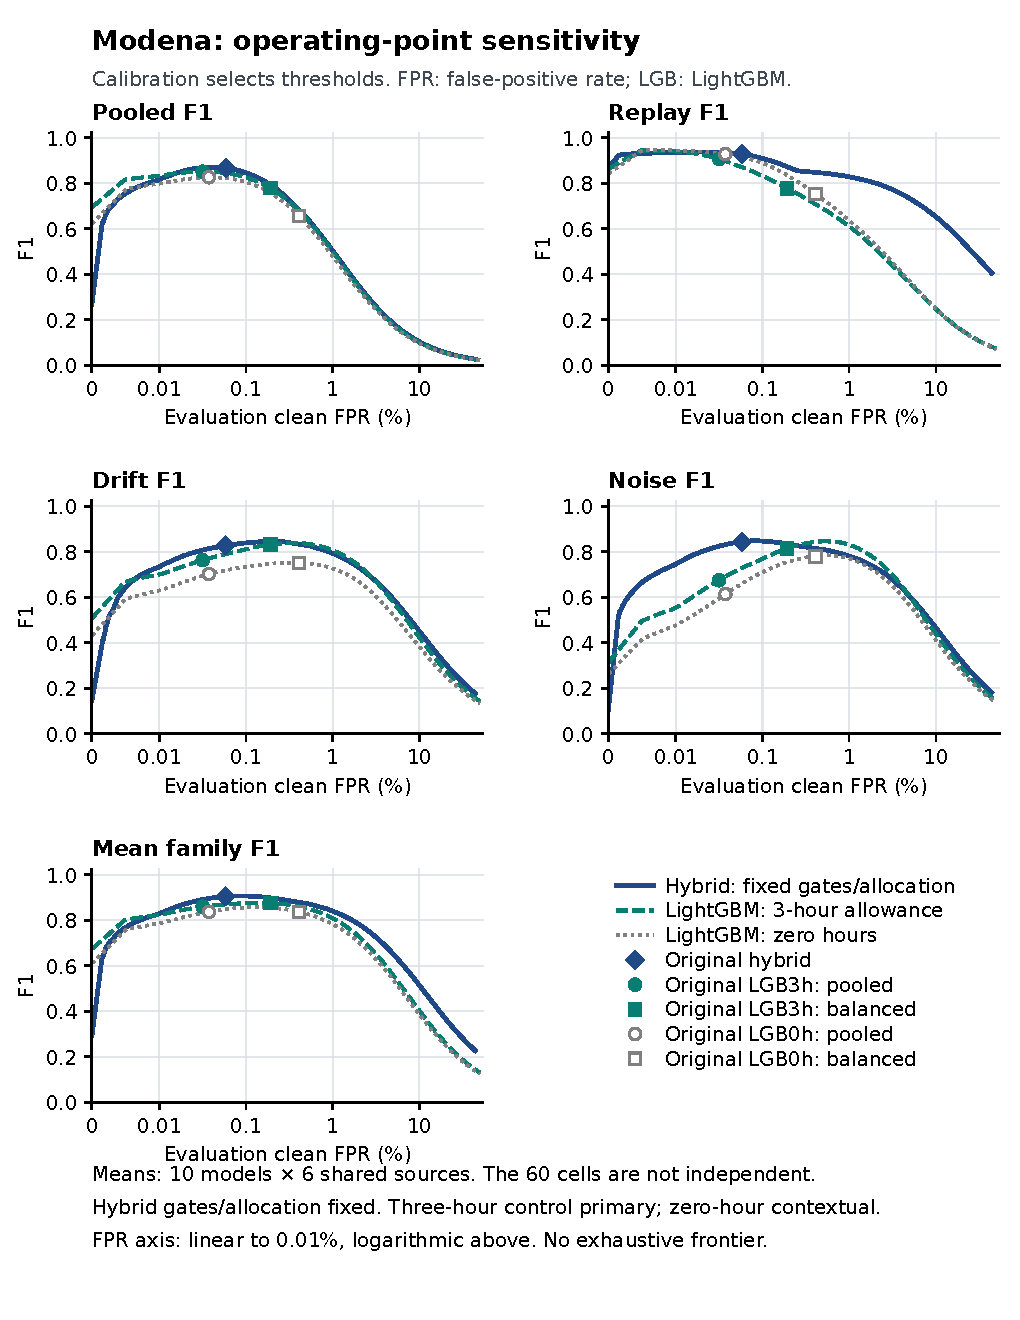
\includegraphics[width=\linewidth,height=.82\textheight,keepaspectratio]{figures/modena_operating_point_sensitivity.pdf}
\caption[Modena operating-point sensitivity]{Modena operating-point sensitivity on the existing evaluation sources. Curves follow the specified calibration-derived threshold paths; symbols mark original operating points. The horizontal axis shows achieved evaluation clean false-positive rate (FPR) in percent, with a linear region up to $0.01\%$ and logarithmic scaling above it. All points are equal-weight means over 60 shared model/source cells. The hybrid path fixes branch allocation and all guard settings.}
\label{fig:modena_operating_sensitivity-supp20261008}
\end{figure}
\begin{figure}[p]
\centering
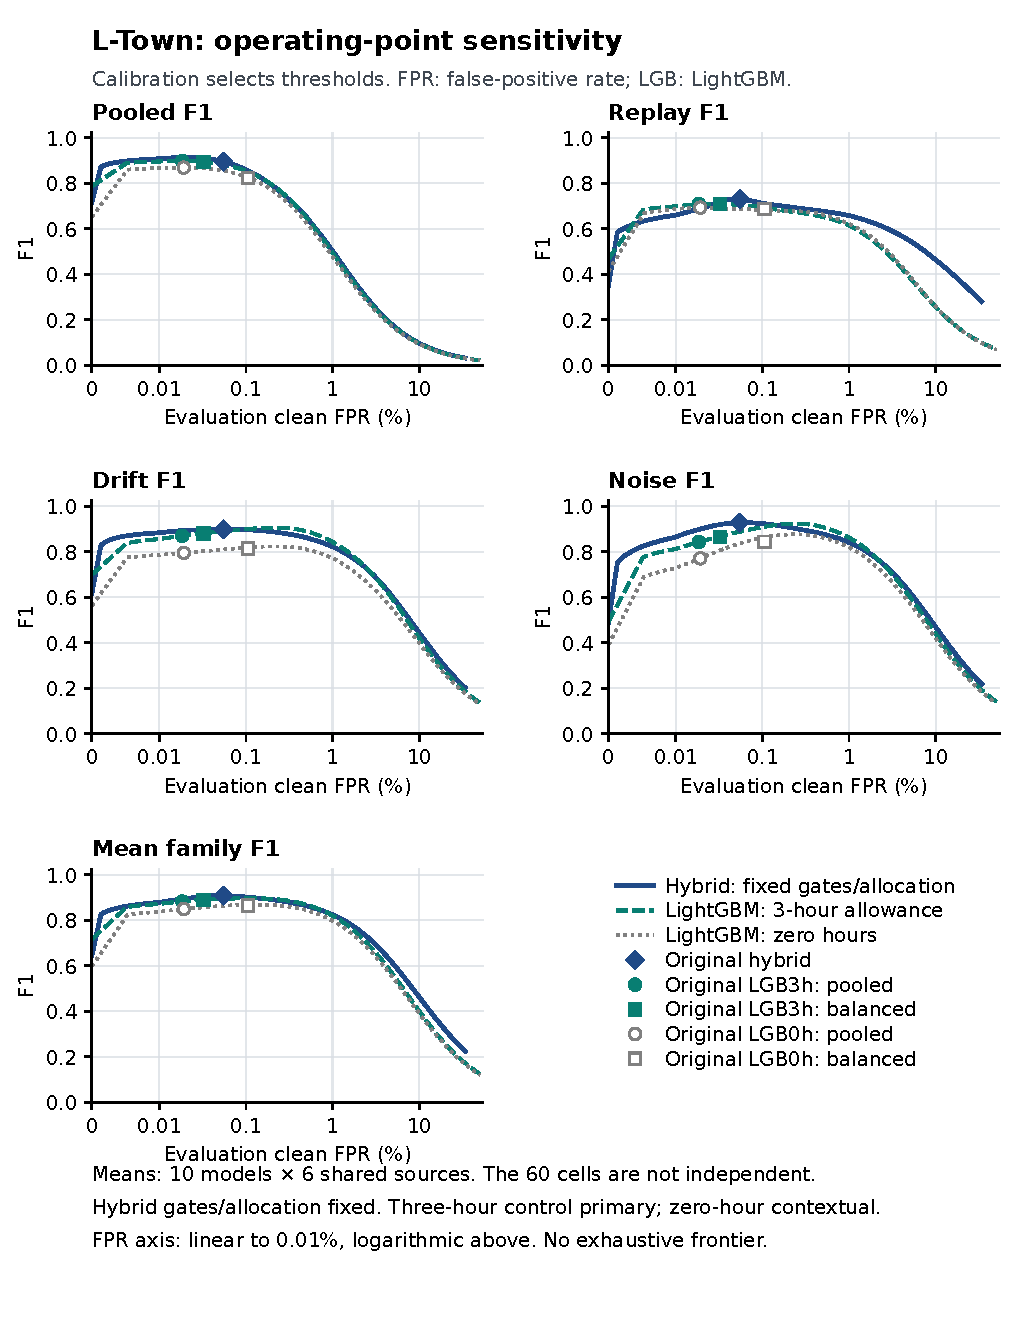
\includegraphics[width=\linewidth,height=.82\textheight,keepaspectratio]{figures/ltown_operating_point_sensitivity.pdf}
\caption[L-Town operating-point sensitivity]{L-Town operating-point sensitivity under the same supplementary protocol. Evaluation clean FPR is observed separately from the calibration cap. The three-hour LightGBM control is primary; the zero-hour control supplies timing context. Curves are finite threshold paths, not an exhaustive hybrid frontier. All points average 60 shared model/source cells.}
\label{fig:ltown_operating_sensitivity-supp20261008}
\end{figure}
\FloatBarrier


\section{Exclusion and iterative reweighting in the pressure reference}
\label{sec:reference_factorial}
The historical reference comparison changed several operations together. A separate $2\times2$ experiment varies target-group exclusion, denoted by $E$, and iteratively reweighted least squares (IRLS), denoted by $R$, within the retained final reference. Values of one enable the operation and zero disable it. The experiment uses model seeds 701--703 and the same six existing evaluation sources per network. The three altered conditions refit the downstream detector; $E=1,R=1$ reuses the corresponding retained models after reference, feature and score checks. All four conditions select thresholds under the same calibration policy. Their comparison therefore concerns adapted detectors with a shared representation, rather than substituting reference features into an unchanged classifier.

The shared reference retains its TRAIN-fitted mean, rank-16 basis, four sensor groups, ridge parameter, inner whitening scale and outer residual scale. All conditions use three views and median aggregation. Disabling exclusion admits observed target-group readings into the snapshot fit while preserving the original non-target view membership. Disabling IRLS reduces six weighted ridge solves to one solve with binary visibility weights. Whitening and median aggregation remain present, so this intervention isolates iterative reweighting rather than removing every source of robustness. Non-target observation support has the same definition in every condition; prediction and view spread are recomputed. Keeping both scales fixed also preserves the normalization and binning of L-Town's received-history features.

The saved full and source-held references preserve their original fitting populations. Modena's full reference uses its earlier 62-scenario TRAIN population, while the downstream detector uses 110 TRAIN scenarios; L-Town uses 120. Six Modena and five L-Town source-held references exclude their respective held source. Each altered condition rebuilds the reference-derived features and refits General, the causal and delayed specialists, the external router and feedback, the early-warning head and the verifiers. L-Town also refits its full-history General mixture. Estimator settings, seed mappings, sampling algorithms and decision-time allowances are unchanged. Later integration layers retain the original source-held stacking procedure, using assembled base out-of-fold predictions. Upstream models are not rebuilt inside every later-layer fold, so the procedure is not fully nested cross-validation.

Calibration follows the 82-point multiplier path in Section~\ref{sec:operating_sensitivity-supp20261008}. Each condition derives its thresholds from its own clean calibration scores, using the original model seed's branch-budget allocation. Final verifier acceptance cutoffs, the external veto and L-Town's routing transformation remain fixed. Verifier candidate prethresholds and early-warning abstention are learned again from the altered condition's TRAIN out-of-fold predictions. The primary policy maximizes pooled F1 under a calibration clean-FPR cap of $0.05\%$. Three secondary policies use worst-family F1 at the same cap and both objectives at $0.50\%$. Ties use the other F1 criterion, lower clean FPR and then the stricter grid setting. The original family-protection constraints are omitted. Evaluation is permitted only after all four policies for all 24 condition/network/model combinations have been fixed.

Metrics are calculated within each model-seed/source cell. The three model-seed values are averaged within each source, followed by equal averaging over six sources. Worst-family F1 is calculated before averaging; descriptive SDs use the six source means. For a metric $M_{ER}$, the exclusion effects are $M_{11}-M_{01}$ with IRLS and $M_{10}-M_{00}$ without it. The IRLS effects are $M_{11}-M_{10}$ with exclusion and $M_{01}-M_{00}$ without it. Their interaction is $M_{11}-M_{10}-M_{01}+M_{00}$. These contrasts are formed within paired cells before averaging. F1 differences are absolute; FPR differences use percentage points. A common calibration cap does not require equal achieved evaluation FPR.

The protocol was fixed before fitting the altered models, after historical outcomes were already known. The stricter cap was chosen to examine the previously observed low-false-alarm range. The study reuses evaluation sources and three retained model seeds, and its fixed branch allocations and gate settings were selected for $E=1,R=1$. These choices limit the comparison to the declared learning recipe and can favor the retained condition. The experiment supplies conditional evidence about exclusion and IRLS; the original selected system and research-goal assessment remain unchanged.

Table~\ref{tab:factorial_primary_modena} reports Modena's primary-policy results. Pooled F1 is 0.8709 with both operations and 0.8752 with IRLS alone, compared with 0.8104 with exclusion alone and 0.8168 with neither. IRLS increases pooled F1 by 0.0606 with exclusion and 0.0584 without it; the corresponding replay gains are 0.3052 and 0.3030. These gains accompany higher evaluation clean FPR. With exclusion enabled, IRLS raises clean FPR from 0.0179\% to 0.0378\%, a difference of 0.0199 percentage points.

The paired effects in Table~\ref{tab:factorial_effects_modena} separate these contributions. Exclusion reduces pooled F1 by 0.0042 with IRLS and 0.0064 without it, with replay differences of $-0.0091$ and $-0.0113$. The pooled-F1 interaction is 0.0022, small relative to the IRLS effects. Thus, within this learning recipe, Modena supports iterative reweighting but does not show a mean pooled-F1 benefit from target-group exclusion. The result also distinguishes the reference's information constraint from an empirical guarantee of improved detection.

% Input summary SHA256: 949d8b4867ba53ef7094144ecc5eb2c620362dd444854cca8f7c10d30a0c9daf
% Calibration fingerprint-map SHA256: 0425957e1aedaaf8b30615d0ced3620c8929d413c4686186e3f8ac31be0e5965
\begin{table}[tbp]
\centering\small
\setlength{\tabcolsep}{4pt}
\renewcommand{\arraystretch}{1.1}
\caption[Modena: primary reference-factorial results]{Modena: primary reference-factorial results. Conditional evaluation means over three model seeds and six shared sources. The primary policy maximizes pooled calibration F1 under a 0.05\% clean-FPR cap. F1 uses the 0--1 scale; achieved evaluation clean FPR is a percentage.}
\label{tab:factorial_primary_modena}
\begin{tabular}{@{}ccrrrrrrr@{}}
\toprule
E & R & Pooled & Random & Replay & Drift & Noise & Targeted & \shortstack{Clean FPR\\(\%)} \\
\midrule
0 & 0 & 0.8168 & 0.9142 & 0.6395 & 0.7934 & 0.7892 & 0.9283 & 0.0170 \\
0 & 1 & 0.8752 & 0.9438 & 0.9425 & 0.8150 & 0.8507 & 0.9577 & 0.0380 \\
1 & 0 & 0.8104 & 0.9038 & 0.6282 & 0.7873 & 0.7860 & 0.9279 & 0.0179 \\
1 & 1 & 0.8709 & 0.9429 & 0.9335 & 0.8144 & 0.8334 & 0.9573 & 0.0378 \\
\bottomrule
\end{tabular}
\par\smallskip
\begin{minipage}{\linewidth}\footnotesize E denotes target-group exclusion and R denotes iterative residual reweighting; 1 is enabled and 0 is disabled. The shared reference representation and scales remain fixed. A calibration cap is not a guarantee of evaluation FPR.\end{minipage}
\end{table}

% Input summary SHA256: 949d8b4867ba53ef7094144ecc5eb2c620362dd444854cca8f7c10d30a0c9daf
% Calibration fingerprint-map SHA256: 0425957e1aedaaf8b30615d0ced3620c8929d413c4686186e3f8ac31be0e5965
\begin{table}[tbp]
\centering\small
\setlength{\tabcolsep}{4pt}
\renewcommand{\arraystretch}{1.1}
\caption[Modena: primary paired factorial effects]{Modena: primary paired factorial effects. Conditional effects under the primary policy, paired within model-seed/source cells. Means average three model seeds within each of six shared sources; SD is the sample standard deviation of the six source means. F1 effects are absolute differences; clean-FPR effects and their SDs are percentage points.}
\label{tab:factorial_effects_modena}
\begin{tabular}{@{}lrrrrrr@{}}
\toprule
Effect & \multicolumn{2}{c}{Pooled F1} & \multicolumn{2}{c}{Replay F1} & \multicolumn{2}{c}{Clean FPR (pp)} \\
\cmidrule(lr){2-3}\cmidrule(lr){4-5}\cmidrule(l){6-7}
 & Mean & SD & Mean & SD & Mean & SD \\
\midrule
Exclusion, IRLS on & -0.0042 & 0.0046 & -0.0091 & 0.0113 & -0.0002 & 0.0051 \\
Exclusion, IRLS off & -0.0064 & 0.0062 & -0.0113 & 0.0148 & +0.0009 & 0.0010 \\
IRLS, exclusion on & +0.0606 & 0.0150 & +0.3052 & 0.0299 & +0.0199 & 0.0043 \\
IRLS, exclusion off & +0.0584 & 0.0110 & +0.3030 & 0.0249 & +0.0210 & 0.0069 \\
Interaction & +0.0022 & 0.0065 & +0.0022 & 0.0200 & -0.0011 & 0.0053 \\
\bottomrule
\end{tabular}
\par\smallskip
\begin{minipage}{\linewidth}\footnotesize Simple effects are enabled minus disabled for the named factor, with the other factor fixed. Interaction is $M_{11}-M_{10}-M_{01}+M_{00}$. Positive F1 differences indicate higher F1; positive FPR differences indicate more false alarms. SD is descriptive, not a standard error.\end{minipage}
\end{table}


L-Town shows a smaller pooled-F1 contribution from IRLS (Table~\ref{tab:factorial_primary_ltown}). Pooled F1 is 0.9129 with both operations and 0.9152 with IRLS alone, compared with 0.9017 with exclusion alone and 0.9011 with neither. The paired IRLS effects are 0.0112 with exclusion and 0.0141 without it. With exclusion enabled, IRLS reduces clean FPR by 0.0042 percentage points; without exclusion, the difference is an increase of 0.0002 percentage points.

Replay reveals an interaction that the pooled means partly conceal (Table~\ref{tab:factorial_effects_ltown}). IRLS changes replay F1 by $-0.0002$ with exclusion and by $+0.0188$ without it, giving an interaction of $-0.0189$. Exclusion changes replay by $-0.0113$ with IRLS and $+0.0077$ without it. Thus, neither operation has a uniform replay effect across reference conditions. Under the primary policy, IRLS alone has the highest mean pooled and replay F1 among the four conditions in both networks, although the fixed learning recipe and reused sources prevent interpreting this as a newly confirmed system selection.

% Input summary SHA256: 949d8b4867ba53ef7094144ecc5eb2c620362dd444854cca8f7c10d30a0c9daf
% Calibration fingerprint-map SHA256: 0425957e1aedaaf8b30615d0ced3620c8929d413c4686186e3f8ac31be0e5965
\begin{table}[tbp]
\centering\small
\setlength{\tabcolsep}{4pt}
\renewcommand{\arraystretch}{1.1}
\caption[L-Town: primary reference-factorial results]{L-Town: primary reference-factorial results. Conditional evaluation means over three model seeds and six shared sources. The primary policy maximizes pooled calibration F1 under a 0.05\% clean-FPR cap. F1 uses the 0--1 scale; achieved evaluation clean FPR is a percentage.}
\label{tab:factorial_primary_ltown}
\begin{tabular}{@{}ccrrrrrrr@{}}
\toprule
E & R & Pooled & Random & Replay & Drift & Noise & Targeted & \shortstack{Clean FPR\\(\%)} \\
\midrule
0 & 0 & 0.9011 & 0.9806 & 0.6801 & 0.8778 & 0.8921 & 0.9784 & 0.0177 \\
0 & 1 & 0.9152 & 0.9941 & 0.6989 & 0.8903 & 0.9038 & 0.9945 & 0.0179 \\
1 & 0 & 0.9017 & 0.9834 & 0.6878 & 0.8859 & 0.9016 & 0.9814 & 0.0234 \\
1 & 1 & 0.9129 & 0.9938 & 0.6876 & 0.8900 & 0.9028 & 0.9942 & 0.0191 \\
\bottomrule
\end{tabular}
\par\smallskip
\begin{minipage}{\linewidth}\footnotesize E denotes target-group exclusion and R denotes iterative residual reweighting; 1 is enabled and 0 is disabled. The shared reference representation and scales remain fixed. A calibration cap is not a guarantee of evaluation FPR.\end{minipage}
\end{table}

% Input summary SHA256: 949d8b4867ba53ef7094144ecc5eb2c620362dd444854cca8f7c10d30a0c9daf
% Calibration fingerprint-map SHA256: 0425957e1aedaaf8b30615d0ced3620c8929d413c4686186e3f8ac31be0e5965
\begin{table}[tbp]
\centering\small
\setlength{\tabcolsep}{4pt}
\renewcommand{\arraystretch}{1.1}
\caption[L-Town: primary paired factorial effects]{L-Town: primary paired factorial effects. Conditional effects under the primary policy, paired within model-seed/source cells. Means average three model seeds within each of six shared sources; SD is the sample standard deviation of the six source means. F1 effects are absolute differences; clean-FPR effects and their SDs are percentage points.}
\label{tab:factorial_effects_ltown}
\begin{tabular}{@{}lrrrrrr@{}}
\toprule
Effect & \multicolumn{2}{c}{Pooled F1} & \multicolumn{2}{c}{Replay F1} & \multicolumn{2}{c}{Clean FPR (pp)} \\
\cmidrule(lr){2-3}\cmidrule(lr){4-5}\cmidrule(l){6-7}
 & Mean & SD & Mean & SD & Mean & SD \\
\midrule
Exclusion, IRLS on & -0.0023 & 0.0011 & -0.0113 & 0.0036 & +0.0012 & 0.0005 \\
Exclusion, IRLS off & +0.0006 & 0.0020 & +0.0077 & 0.0042 & +0.0057 & 0.0008 \\
IRLS, exclusion on & +0.0112 & 0.0013 & -0.0002 & 0.0070 & -0.0042 & 0.0009 \\
IRLS, exclusion off & +0.0141 & 0.0019 & +0.0188 & 0.0070 & +0.0002 & 0.0004 \\
Interaction & -0.0029 & 0.0024 & -0.0189 & 0.0049 & -0.0045 & 0.0009 \\
\bottomrule
\end{tabular}
\par\smallskip
\begin{minipage}{\linewidth}\footnotesize Simple effects are enabled minus disabled for the named factor, with the other factor fixed. Interaction is $M_{11}-M_{10}-M_{01}+M_{00}$. Positive F1 differences indicate higher F1; positive FPR differences indicate more false alarms. SD is descriptive, not a standard error.\end{minipage}
\end{table}


Appendix~\ref{app:reference_factorial} reports all four calibration policies. Relaxing the clean-FPR cap from $0.05\%$ to $0.50\%$ leaves the pooled-objective evaluation summaries unchanged. Changing the objective has a larger effect. For L-Town with both reference operations, worst-family calibration at the stricter cap raises replay F1 from 0.6876 to 0.7293, while pooled F1 falls from 0.9129 to 0.9015 and clean FPR rises from 0.0191\% to 0.0462\%. These comparisons support a contribution from IRLS to pooled performance, especially in Modena, but do not establish a consistent benefit from exclusion or a replay improvement independent of calibration policy. The complete counts, contrasts and frozen implementation are available in evidence record \evid{E11}.

\endgroup
